\documentclass[12pt, a4paper]{extarticle}
\usepackage{GOST}
\usepackage{array}
\usepackage{verbatim}
\usepackage[detect-all]{siunitx}
\usepackage{amsmath}
\usepackage{amssymb}
\usepackage[utf8]{inputenc}
\usepackage{hyperref}
\usepackage{tempora}

\makeatletter
\renewcommand\@biblabel[1]{#1.}
\makeatother

\usepackage{listings}
\lstset{ 
	language=Prolog,
	basicstyle=\small, 
	numbers=left, 
	numberstyle=\tiny,
	stepnumber=1,
	numbersep=5pt,
	showspaces=false,            
	showstringspaces=false,      
	showtabs=false,             
	frame=single,            % рисовать рамку вокруг кода
	tabsize=4,      
	commentstyle=\color{green},
	keywordstyle=\color{blue}\textbf,
	numberstyle=\scriptsize\color{gray}, % the style that is used for the line-numbers
	rulecolor=\color{black},
	captionpos=t,
	breaklines=true,         % автоматически переносить строки 
	breakatwhitespace=false, % переносить строки по пробелу
	%escapeinside={\#*}{*)} 
}



\begin{document}
	
\begin{table}[ht]
	\centering
	\begin{tabular}{|c|p{400pt}|} 
		\hline
		\begin{tabular}[c]{@{}c@{}} 
\includegraphics[scale=1]{source/b_logo.jpg} \\\end{tabular} &
		\footnotesize\begin{tabular}[c]{@{}c@{}}\textbf{Министерство~науки~и~высшего~образования~Российской~Федерации}\\\textbf{Федеральное~государственное~бюджетное~образовательное~учреждение}\\\textbf{~высшего~образования}\\\textbf{«Московский~государственный~технический~университет}\\\textbf{имени~Н.Э.~Баумана}\\\textbf{(национальный~исследовательский~университет)»}\\\textbf{(МГТУ~им.~Н.Э.~Баумана)}\\\end{tabular}  \\
		\hline
	\end{tabular}
\end{table}
\noindent\rule{\textwidth}{4pt}
\noindent\rule[14pt]{\textwidth}{1pt}
\hfill 
\noindent
\makebox{ФАКУЛЬТЕТ~}%
\makebox[\textwidth][l]{\underline{~«Информатика и системы управления»~~~~~~~~~~~~~~~~~~~~~~~~~~~~~~~~~}}%
\\
\noindent
\makebox{КАФЕДРА~}%
\makebox[\textwidth][l]{\underline{~«Программное обеспечение ЭВМ и информационные технологии»~}}%
\\

\begin{center}
	\vspace{1.5cm}
	{\bf\huge Отчёт\par}
	{\bf\Large по лабораторной работе № 18\par}
	\vspace{0.7cm}
\end{center}


\noindent
\makebox{\large{\bf Название:}~~~}
\makebox[\textwidth][l]{\large\underline{~Формирование эффективных программ на Prolog~}}\\

\noindent
\makebox{\large{\bf Дисциплина:}~~~}
\makebox[\textwidth][l]{\large\underline{~Функциональное и логическое программирование~}}\\

\vspace{1.5cm}
\noindent
\begin{tabular}{l c c c c c}
	Студент      & ~ИУ7-65Б~               & \hspace{2.5cm} & \hspace{2cm}                 & &  Д.В. Сусликов \\\cline{2-2}\cline{4-4} \cline{6-6} 
	\hspace{3cm} & {\footnotesize(Группа)} &                & {\footnotesize(Подпись, дата)} & & {\footnotesize(И.О. Фамилия)}
\end{tabular}

\noindent
\begin{tabular}{l c c c c}
	Преподаватель & \hspace{5cm}   & \hspace{2cm}                 & & ~~~~~~Н.Б. Толпинская~~~~~~\\\cline{3-3} \cline{5-5} 
	\hspace{3cm}  &                & {\footnotesize(Подпись, дата)} & & {\footnotesize(И.О. Фамилия)}
\end{tabular}

\vspace{0.6cm}
\begin{center}	
	\vfill
	\large \textit {Москва, 2021}
\end{center}

\thispagestyle {empty}
\pagebreak

\clearpage

\textbf{Задание}

Используя хвостовую рекурсию, разработать программу, позволяющую найти 

\begin{enumerate}
	\item n!
	\item n-е число Фибоначчи
\end{enumerate}

Убедиться в правильности результатов.

Для одного из вариантов вопроса и каждого задания составить таблицу, отражающую конкретный порядок работы системы


\hfill

\textbf{Листинг факториала:}

\begin{lstlisting}
	predicates
		fact(integer, integer, integer).	
	clauses
		fact(1, R, R) :- !.
		fact(N, Acc, R):-
			New_N = N - 1,
			New_Acc = Acc * N,
			fact(New_N, New_Acc, R).		
	goal
		fact(3, 1, Result). 
\end{lstlisting}
\par

\textbf{Листинг фибоначчи:}
\begin{lstlisting}
predicates
	fibb(integer,integer,integer,integer)
clauses
	fibb(1, _, Res, Res):- !.
	fibb(I, Last, Cur, Res):- 
		NI = I - 1,
		NLast = Cur,
		NCur = Last + Cur,
		fibb(NI, NLast, NCur, Res).
goal
	fibb(5, 0, 1, R).
\end{lstlisting}
\newpage

Результаты работы:\par
\begin{figure}[h!]
	\begin{minipage}[h]{0.48\linewidth}
		\center{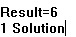
\includegraphics[width=0.48\linewidth]{source/1.png} \\ Пример fac}	
	\end{minipage}
	\hfill
	\begin{minipage}[h]{0.48\linewidth}
		\center{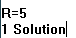
\includegraphics[width=0.48\linewidth]{source/2.png} \\ Пример fibb}	
	\end{minipage}
\end{figure}\par

\newpage
\textbf{Приведем таблицу для нахождения факториала. }\par
fact(3, 1, R)\par

\begin{table}[h!]
	\begin{tabular}{|l|l|l|l|}
		\hline
		\begin{tabular}[c]{@{}l@{}}№\\ шага\end{tabular} & \begin{tabular}[c]{@{}l@{}}Состояние резольвенты\\ и вывод\end{tabular}                                  & \begin{tabular}[c]{@{}l@{}}Для каких термов запускается\\ алгоритм унификации и\\ каков результат\end{tabular}                                          & Дальнейшие действия                                                             \\ \hline
		0                                                & fact(3, 1, R)                                                                                            &                                                                                                                                                         &                                                                                 \\ \hline
		1                                                & fact(3, 1, R)                                                                                            & \begin{tabular}[c]{@{}l@{}}T1 =  fact(3, 1, R)\\ T2 = fact(1, \_, R).\\ Неудача. Не унифицируемы\end{tabular}                                           & \begin{tabular}[c]{@{}l@{}}Переход к следующему\\ заголовку БЗ\end{tabular}     \\ \hline
		2                                                & fact(3, 1, R)                                                                                            & \begin{tabular}[c]{@{}l@{}}Т1 = fact(3, 1, R)\\ Т2 = fact(N, Acc, R)\\ Успех. Унифицируемы.\\ \\ Подстановка:\\ \{N = 3,  Acc = 1, R = R\}\end{tabular} & \begin{tabular}[c]{@{}l@{}}Замена на тело\\ предложения\end{tabular}            \\ \hline
		3                                                & \begin{tabular}[c]{@{}l@{}}New\_N = 3 - 1,\\ New\_Acc = 1 * 3,\\ fact(New\_N, New\_Acc, R).\end{tabular} & \begin{tabular}[c]{@{}l@{}}New\_N =  3 - 1\\ New\_N = 2\end{tabular}                                                                                    & \begin{tabular}[c]{@{}l@{}}Замена на тело\\ предложения\\ (пустое)\end{tabular} \\ \hline
		4                                                & \begin{tabular}[c]{@{}l@{}}New\_Acc = 1 * 3,\\ fact(2, New\_Acc, R).\end{tabular}                        & \begin{tabular}[c]{@{}l@{}}New\_Acc = 1 * 3\\ New\_Acc = 3\end{tabular}                                                                                 & \begin{tabular}[c]{@{}l@{}}Замена на тело\\ предложения\\ (пустое)\end{tabular} \\ \hline
		5                                                & fact(2, 3, R).                                                                                           & \begin{tabular}[c]{@{}l@{}}T1 = fact(2, 3, R)\\ T2 = fact(1, \_, R).\\ Неудача. Не унифицируемы.\end{tabular}                                           & \begin{tabular}[c]{@{}l@{}}Переход к следующему\\ заголовку БЗ\end{tabular}     \\ \hline
		6                                                & fact(2, 3, R).                                                                                           & \begin{tabular}[c]{@{}l@{}}T1 = fact(2, 3, R)\\ T2 = fact(N, Acc, R)\\ Успех. Унифицируемы.\\ \\ Подстановка:\\ \{N = 2,  Acc = 3, R = R\}\end{tabular} & \begin{tabular}[c]{@{}l@{}}Замена на тело\\ предложения\end{tabular}            \\ \hline
	\end{tabular}
\end{table}
\newpage

\begin{table}[h!]
	\begin{tabular}{|l|l|l|l|}
		\hline
		7  & \begin{tabular}[c]{@{}l@{}}New\_N = 2 - 1,\\ New\_Acc = 3 * 2,\\ fact(New\_N, New\_Acc, R).\end{tabular} & \begin{tabular}[c]{@{}l@{}}New\_N = 2 - 1\\ New\_N = 1\end{tabular}                                                                                 & \begin{tabular}[c]{@{}l@{}}Замена на тело\\ предложения\\ (пустое)\end{tabular} \\ \hline
		8  & \begin{tabular}[c]{@{}l@{}}New\_Acc = 3 * 2,\\ fact(1, New\_Acc, R).\end{tabular}                        & \begin{tabular}[c]{@{}l@{}}New\_Acc = 3 * 2\\ New\_Acc = 6\end{tabular}                                                                             & \begin{tabular}[c]{@{}l@{}}Замена на тело\\ предложения\\ (пустое)\end{tabular} \\ \hline
		9  & fact(1, 6, R)                                                                                            & \begin{tabular}[c]{@{}l@{}}T1 = fact(1, 6, R)\\ T2 = fact(1, \_, R)\\ Успех. Унифицируемы.\\ \\ Подстановка:\\ \{1 = 1, R = 6, R = R\}\end{tabular} & \begin{tabular}[c]{@{}l@{}}Замена на тело\\ предложения\end{tabular}            \\ \hline
		10 & !                                                                                                        & \begin{tabular}[c]{@{}l@{}}!\\ Истина\end{tabular}                                                                                                  & \begin{tabular}[c]{@{}l@{}}Замена на тело\\ предложения\\ (пустое)\end{tabular} \\ \hline
		11 & \begin{tabular}[c]{@{}l@{}}Вывод\\ R = 6\\ \\ Резольвента пуста\end{tabular}                             &                                                                                                                                                     & Откат.                                                                          \\ \hline
		12 & !                                                                                                        & \begin{tabular}[c]{@{}l@{}}!\\ Завершение процедуры\end{tabular}                                                                                    & \begin{tabular}[c]{@{}l@{}}Замена на тело\\ предложения\\ (пустое)\end{tabular} \\ \hline
		13 & Резольвента пуста                                                                                        &                                                                                                                                                     & \begin{tabular}[c]{@{}l@{}}Завершение работы\\ программы\end{tabular}           \\ \hline
	\end{tabular}
\end{table}

\newpage

\textbf{Приведем таблицу для нахождения числа полследовательности Фибоначчи. }\par
fibb(3, 0, 1, Res)\par

\begin{table}[h!]
	\begin{tabular}{|l|l|l|l|}
		\hline
		\begin{tabular}[c]{@{}l@{}}№\\ шага\end{tabular} & \begin{tabular}[c]{@{}l@{}}Состояние резольвенты\\ и вывод\end{tabular}                                        & \begin{tabular}[c]{@{}l@{}}Для каких термов запускается\\ алгоритм унификации и\\ каков результат\end{tabular}                                                                     & Дальнейшие действия                                                             \\ \hline
		0                                                & fibb(3, 0, 1, Res)                                                                                             &                                                                                                                                                                                    &                                                                                 \\ \hline
		1                                                & fibb(3, 0, 1, Res)                                                                                             & \begin{tabular}[c]{@{}l@{}}T1 =  fibb(3, 0, 1, Res)\\ T2 = fibb(1, \_, Res, Res)\\ Неудача. Не унифицируемы\end{tabular}                                                           & \begin{tabular}[c]{@{}l@{}}Переход к следующему\\ заголовку БЗ\end{tabular}     \\ \hline
		2                                                & fibb(3, 0, 1, Res)                                                                                             & \begin{tabular}[c]{@{}l@{}}T1 = fibb(3, 0, 1, Res)\\ T2 =  fibb(I, Last, Cur, Res)\\ Успех. Унифицируемы.\\ \\ Подстановка:\\ \{I = 3, Last = 0, Cur = 1, Res = Res\}\end{tabular} & \begin{tabular}[c]{@{}l@{}}Замена на тело\\ предложения\end{tabular}            \\ \hline
		3                                                & \begin{tabular}[c]{@{}l@{}}NI = 3 - 1,\\ NLast = 1,\\ NCur = 0 + 1,\\ fibb(NI, NLast, NCur, Res).\end{tabular} & \begin{tabular}[c]{@{}l@{}}NI = 3 - 1\\ NI = 2\end{tabular}                                                                                                                        & \begin{tabular}[c]{@{}l@{}}Замена на тело\\ предложения\\ (пустое)\end{tabular} \\ \hline
		4                                                & \begin{tabular}[c]{@{}l@{}}NLast = 1,\\ NCur = 0 + 1,\\ fibb(2, NLast, NCur, Res)\end{tabular}                 & NLast = 1                                                                                                                                                                          & \begin{tabular}[c]{@{}l@{}}Замена на тело\\ предложения\\ (пустое)\end{tabular} \\ \hline
		5                                                & \begin{tabular}[c]{@{}l@{}}NCur = 0 + 1,\\ fibb(2, 1, NCur, Res)\end{tabular}                                  & \begin{tabular}[c]{@{}l@{}}NCur = 0 + 1\\ NCur = 1\end{tabular}                                                                                                                    & \begin{tabular}[c]{@{}l@{}}Замена на тело\\ предложения\\ (пустое)\end{tabular} \\ \hline
		6                                                & fibb(2, 1, 1, Res)                                                                                             & \begin{tabular}[c]{@{}l@{}}T1 = fibb(2, 1, 1, Res)\\ T2 = fibb(1, \_, Res, Res)\\ Неудача. Не унифицируемы.\end{tabular}                                                           & \begin{tabular}[c]{@{}l@{}}Переход к следующему\\ заголовку БЗ\end{tabular}     \\ \hline
	\end{tabular}
\end{table}


\begin{table}[]
	\begin{tabular}{|l|l|l|l|}
		\hline 7                                                & fibb(2, 1, 1, Res)                                                                                             & \begin{tabular}[c]{@{}l@{}}T1 = fibb(2, 1, 1, Res)\\ T2 =  fibb(I, Last, Cur, Res)\\ Успех. Унифицируемы.\\ \\ Подстановка:\\ \{I = 2, Last = 1, Cur = 1, Res = Res\}\end{tabular} & \begin{tabular}[c]{@{}l@{}}Замена на тело\\ предложения\end{tabular}            \\ 
		\hline
		8  & \begin{tabular}[c]{@{}l@{}}NI = 2 - 1,\\ NLast = 1,\\ NCur = 1 + 1,\\ fibb(NI, NLast, NCur, Res).\end{tabular} & \begin{tabular}[c]{@{}l@{}}NI = 2 - 1\\ NI = 1\end{tabular}                                                                                                                 & \begin{tabular}[c]{@{}l@{}}Замена на тело\\ предложения\\ (пустое)\end{tabular} \\ \hline
		9  & \begin{tabular}[c]{@{}l@{}}NLast = 1,\\ NCur = 1 + 1,\\ fibb(1, NLast, NCur, Res).\end{tabular}                & NLast = 1                                                                                                                                                                   & \begin{tabular}[c]{@{}l@{}}Замена на тело\\ предложения\\ (пустое)\end{tabular} \\ \hline
		10 & \begin{tabular}[c]{@{}l@{}}NCur = 1 + 1,\\ fibb(1, 1, NCur, Res).\end{tabular}                                 & \begin{tabular}[c]{@{}l@{}}NCur = 1 + 1\\ NCur = 2\end{tabular}                                                                                                             & \begin{tabular}[c]{@{}l@{}}Замена на тело\\ предложения\\ (пустое)\end{tabular} \\ \hline
		11 & fibb(1, 1, 2, Res)                                                                                             & \begin{tabular}[c]{@{}l@{}}T1 = fib(1, 1, 2, Res)\\ T2 = fib(1, \_, Res, Res)\\ Успех. Унифицируемы.\\ \\ Подстановка:\\ \{1 = 1, \_ = 1, Res = 2, Res = Res\}\end{tabular} & \begin{tabular}[c]{@{}l@{}}Замена на тело\\ предложения\end{tabular}            \\ \hline
		12 & !                                                                                                              & \begin{tabular}[c]{@{}l@{}}!\\ Истина\end{tabular}                                                                                                                          & \begin{tabular}[c]{@{}l@{}}Замена на тело\\ предложения\\ (пустое)\end{tabular} \\ \hline
		13 & \begin{tabular}[c]{@{}l@{}}Вывод\\ Res = 2\\ Резольвента пуста\end{tabular}                                    &                                                                                                                                                                             & Откат                                                                           \\ \hline
		14 & !                                                                                                              & \begin{tabular}[c]{@{}l@{}}!\\ Завершение процедуры\end{tabular}                                                                                                            & \begin{tabular}[c]{@{}l@{}}Замена на тело\\ предложения\\ (пустое)\end{tabular} \\ \hline
		15 & Резольвента пуста                                                                                              &                                                                                                                                                                             & \begin{tabular}[c]{@{}l@{}}Завершение работы\\ программы\end{tabular}           \\ \hline
	\end{tabular}
\end{table} \par

\newpage

\textbf{Вывод}\par
Эффективность работы системы может быть достигнута за счет хвостовой
рекурсии и использования отсечения в тех
случаях, где заведомо известна единственность ответа на вопрос.


\textbf{Ответы на вопросы}
\begin{itemize}
	\item[1)] Что такое рекурсия? Как организуется хвостовая рекурсия в Prolog? Как организовать выход из рекурсии в Prolog?\par	
	Рекурсия – определение объекта через ссылку на самого себя. Один из
	способов организации повторных вычислений. Для организации хвостовой рекурсии необходимо, чтобы рекурсивный вызов был последним в теле рекурсивного правила, и не оставалось других точек выбора. Выход из рекурсии осуществляется либо достижением базиса рекурсии, либо условием в теле правила.
	
	\item[2)] Какое первое состояние резольвенты?\par
	Исходная резольвента содержит вопрос.
	
	\item[3)] В каком случае система запускает алгоритм унификации? (Как эту необходимость на формальном уровне распознает система?)\par
	
	Система запускает алгоритм унификации, когда резольвента не пуста.
	
	\item[4)] В каких пределах программы уникальны переменные?\par
	Именованные переменные уникальны в рамках предложения, анонимные - уникальны везде.
	
	\item[5)] Как применяется подстановка, полученная с помощью алгоритма
	унификации?\par	
	В результате подстановки связываются переменные, которые еще не были
	связаны. После связывания всех утверждений, будет напечатано значение
	связанных переменных.
	
	\item[6)] Как формируется новое состояние резольвенты?\par
	Резольвента меняется в 2 этапа:
	\begin{itemize}
		\item Редукция (замена вопроса на тело правила, заголовок которого был успешно унифицирован);
		\item Применение подстановки.
	\end{itemize}
	
	\item[7)] В каких случаях запускается механизм отката?\par
	В случае, когда унификация на текущем шаге завершается тупиковой
	ситуацией, или был получен ответ «да».
\end{itemize}

\end{document}